\hspace{0.5 cm}
Pentru rularea benchmark-ului cGan am ales ca și tool-uri  alpha\textunderscore beta\textunderscore crown si NeuralSAT, verificând prima dată cu atenție dacă acestea au putut rula setul de date, figura \ref{cGan_gr}. Am facut această alegere deoarece am dorit o comparație dintre primul tool care a obțiunut un timp de verificare mai eficient, iar cel de al doilea care a obținut cel mai ineficient timp de verificare.

\begin{figure}[ht]
\centering
{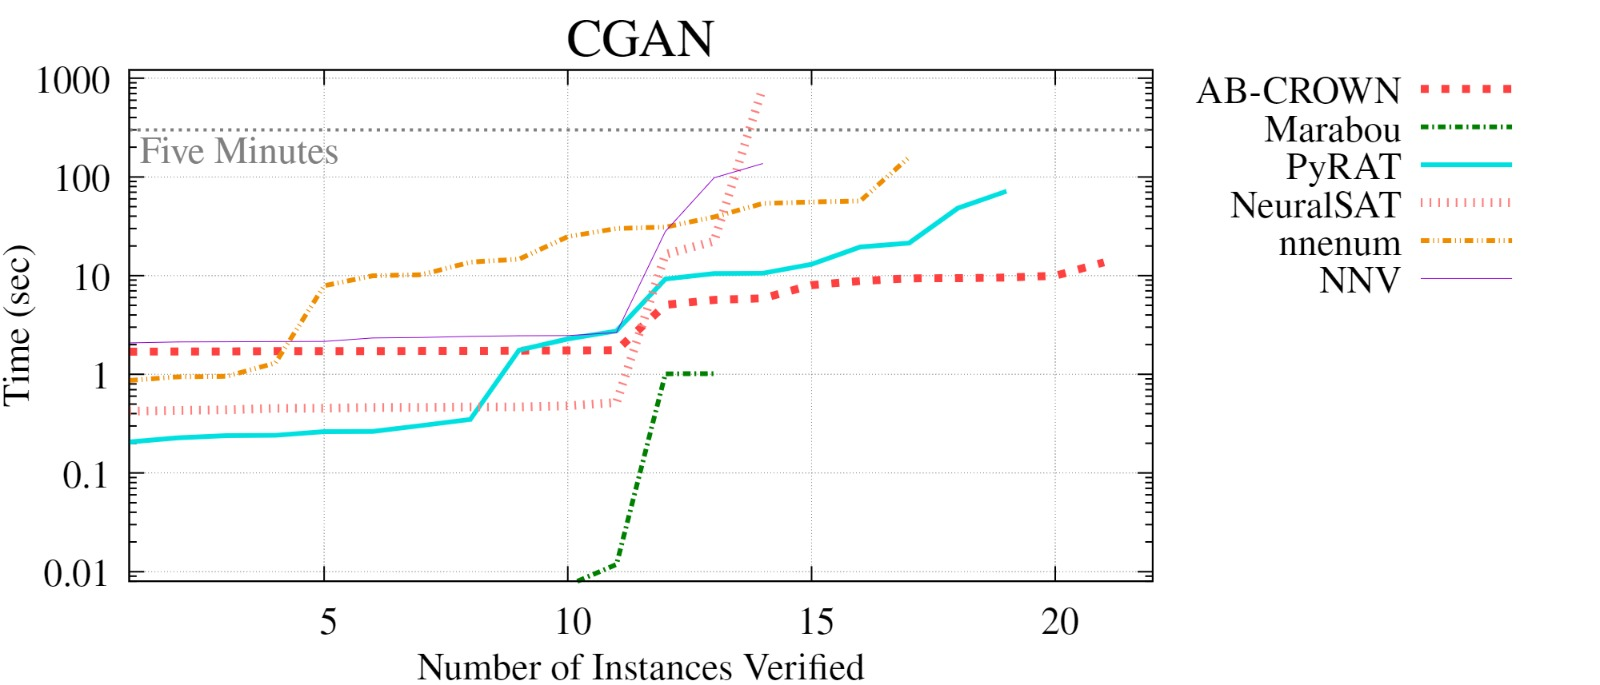
\includegraphics[width=12cm]{imagini/cGan_grafic.jpg}}
\caption{Rezultatele rulării tool-urilor pentru benchmark-ul cGan}
\label{cGan_gr}
\end{figure}

Alpha\textunderscore beta\textunderscore CROWN a fost testat pe Python 3.11, sistemul de operare utilizat a fost  Ubuntu 20.04 prin Windows Subsystem for Linux (WSL) pe Windows 10, folosind un GPU de laptop NVIDIA GeForce RTX 3060.  A fost instalat într-un mediu miniconda. În urmatorii pasi se va explica cum a fost facută instalarea și rularea tool-ului.


\subsection*{Pai de Instalare:}

\begin{enumerate}
  \item Instalarea Miniconda a fost realizată prin linia de comandă (bash) cu următorii pași:
  \begin{lstlisting}[style=bashstyle]
    mkdir -p ~/miniconda3
    wget https://repo.anaconda.com/miniconda/Miniconda3-
    latest-Linux-x86_64.sh -O ~/miniconda3/miniconda.sh
    bash ~/miniconda3/miniconda.sh -b -u -p ~/miniconda3
    rm -rf ~/miniconda3/miniconda.sh
    ~/miniconda3/bin/conda init bash
   \end{lstlisting}
  
  \item Clonarea repository-ului de la adresa \cite{crownrepository}:
    \begin{lstlisting}[style=bashstyle]
    git clone --recursive https://github.com/Verified-
    Intelligence/alpha-beta-CROWN.git
   \end{lstlisting}
  
  \item Clonarea submodulului \texttt{auto\_Lirpa} în interiorul directorului \texttt{alpha-beta-CROWN}:
    \begin{lstlisting}[style=bashstyle]
    git clone https://github.com/Verified-
    Intelligence/auto_LiRPA.git alpha-beta-CROWN/auto_LiRPA
   \end{lstlisting}
  
  \item Configurarea mediului Conda:
    \begin{lstlisting}[style=bashstyle]
    conda deactivate; conda env remove --name alpha-beta-crown
    conda env create -f complete_verifier/environment.yaml --name alpha-beta-crown
    conda activate alpha-beta-crown
   \end{lstlisting}
  
  \item Crearea directorului \texttt{vnncomp2023\_benchmarks} și clonarea repository-ului \cite{cganrepository} în interiorul acestuia. Modificarea \textbf{root path-ului} în fișierul \texttt{cgan.yaml} conform locației reale a directorului \texttt{cgan}.
  
  \item Rularea verificatorului:
  \begin{lstlisting}[style=bashstyle]
    python abcrown.py --config exp_configs/vnncomp23/cgan.yaml
  \end{lstlisting}
  
  \item Pentru a rezolva eroarea legată de \texttt{libcudnn\_cnn\_infer.so.8}, adăugarea următoarei linii în \texttt{.bashrc}:
  \begin{lstlisting}[style=bashstyle]
    export LD_LIBRARY_PATH=/usr/lib/wsl/lib:$LD_LIBRARY_PATH
  \end{lstlisting}
  
  \item Rerularea comenzii și salvarea rezultatelor în \texttt{results.txt}:
  \begin{lstlisting}[style=bashstyle]
    python abcrown.py --config exp_configs/vnncomp23/cgan.yaml > results.txt
  \end{lstlisting}
\end{enumerate}

Cel mai dificil pas a fost remedierea erorii legate de libraria libcudnn\textunderscore cnn\textunderscore infer.so.8., fiind si pasul care a durat cel mai mult timp. Am rezolvat aceasta eroare folosind multiple sugestii gasite pe diferite platforme online \cite{bashrcfix}.